Bevor die Anfangswerte zur globalen Beleuchtung benutzt werden (siehe auch \nameref{pic:Render Graph}), durchlaufen Sie nach dem Sortieren 
(siehe \ref{ch:Content2:sec:Sorting}) das Retargeting. Der Sinn liegt hierbei beim Vertauschen der Anfangswerte, sodass Sie 
verteilt sind wie $BlueNoise_{t+1}$. Aufgrund dessen ergibt sich eine bessere Aufsummierung der
\nameref{ch:Content1:sec:blue noise} Fehlerverteilungen über die ersten paar Bilder.
\par 

\begin{figure}[H]
    \begin{tcolorbox}[boxrule=4pt,sharp corners=downhill,title=Bedeutung des Retargeting]
    %%%%%%%%%%%%%%%%%%%%%%%%%%%%%%%%%%%%%%%%%%%%%%%%%%%%%%%%%%%%%%%%%%%%%%%%%%%%%%%%%%%%%%%%%%%%%%%%%%%%%%
    %%%%%%%%%%%%%%%%%%%%%%%%%%%%%%% second row --> sorting block size 2 without retargeting
    %%%%%%%%%%%%%%%%%%%%%%%%%%%%%%%%%%%%%%%%%%%%%%%%%%%%%%%%%%%%%%%%%%%%%%%%%%%%%%%%%%%%%%%%%%%%%%%%%%%%%%
    \paragraph{\hfill\colorbox{blue}{\textcolor{white}{nur Sorting}}}
    \centering
    \begin{subfigure}[b]{0.2\linewidth}
      
\includegraphics[width=\linewidth]{content/TemporalerAlg/Bilder/Retargeting/Bedeutung Retargeting/Sorting_Small_Block/Spektrum/Ausschnitt1.png}
       \caption{FT t = 0}
       \label{pic:sortier_t0}
    \end{subfigure}
    \begin{subfigure}[b]{0.2\linewidth}
      
\includegraphics[width=\linewidth]{content/TemporalerAlg/Bilder/Retargeting/Bedeutung Retargeting/Sorting_Small_Block/Spektrum/Ausschnitt2.png}
      \caption{FT t = 1}
      \label{pic:sortier_t1}
    \end{subfigure}
    \begin{subfigure}[b]{0.2\linewidth}
      
\includegraphics[width=\linewidth]{content/TemporalerAlg/Bilder/Retargeting/Bedeutung Retargeting/Sorting_Small_Block/Ausschnitt/Ausschnitt3.png}
      \caption{t=2}
      \label{pic:sortier_screen_t2}
    \end{subfigure}
    \begin{subfigure}[b]{0.2\linewidth}
        
\includegraphics[width=\linewidth]{content/TemporalerAlg/Bilder/Retargeting/Bedeutung Retargeting/Sorting_Small_Block/Spektrum/Ausschnitt3.png}
        \caption{FT t = 2}
        \label{pic:sortier_t2}
      \end{subfigure}
    %%%%%%%%%%%%%%%%%%%%%%%%%%%%%%%%%%%%%%%%%%%%%%%%%%%%%%%%%%%%%%%%%%%%%%%%%%%%%%%%%%%%%%%%%%%%%%%%%%%%%%
    %%%%%%%%%%%%%%%%%%%%%%%%%%%%%%% second row --> sorting block size 2 with retargeting
    %%%%%%%%%%%%%%%%%%%%%%%%%%%%%%%%%%%%%%%%%%%%%%%%%%%%%%%%%%%%%%%%%%%%%%%%%%%%%%%%%%%%%%%%%%%%%%%%%%%%%%
    \tcblower
    \paragraph{\hfill\colorbox{blue}{\textcolor{white}{Sorting + Retargeting}}}
    \centering
    \begin{subfigure}[b]{0.2\linewidth}
        
\includegraphics[width=\linewidth]{content/TemporalerAlg/Bilder/Retargeting/Bedeutung Retargeting/Sorting_Small_Block_WithRetargeting/Spektrum/Ausschnitt1.png}
         \caption{FT t = 0}
         \label{pic:retarget_t0}
    \end{subfigure}
    \begin{subfigure}[b]{0.2\linewidth}
        
\includegraphics[width=\linewidth]{content/TemporalerAlg/Bilder/Retargeting/Bedeutung Retargeting/Sorting_Small_Block_WithRetargeting/Spektrum/Ausschnitt2.png}
         \caption{FT t = 1}
         \label{pic:retarget_t1}
    \end{subfigure}
    \begin{subfigure}[b]{0.2\linewidth}
        
\includegraphics[width=\linewidth]{content/TemporalerAlg/Bilder/Retargeting/Bedeutung Retargeting/Sorting_Small_Block_WithRetargeting/Ausschnitt/Ausschnitt3.png}
         \caption{t=2}
         \label{pic:retarget_screen_t2}
    \end{subfigure}
    \begin{subfigure}[b]{0.2\linewidth}
        
\includegraphics[width=\linewidth]{content/TemporalerAlg/Bilder/Retargeting/Bedeutung Retargeting/Sorting_Small_Block_WithRetargeting/Spektrum/Ausschnitt3.png}
         \caption{FT t = 2}
         \label{pic:retarget_t2}
    \end{subfigure}
    \end{tcolorbox}
    \caption{Vergleich erste Bilder Sorting(B=2) mit bzw. ohne Retargeting}
    \label{fig:VergleichRetargetSorting}
\end{figure}

Die Abbildung \ref{fig:VergleichRetargetSorting} verdeutlicht die Bedeutung des Retargeting 
Schrittes. Sie zeigen dieselben Ausschnitte eines homogenen Szenenausschnitts bzw. die korrespondierende 
Spektra über die ersten drei Bilder. Die erste Reihe mit den Bildern

\begin{itemize}
    \item[a.) - d.)] zeigt auch nach dem dritten Bild keine \nameref{ch:Content1:sec:blue noise} Eigenschaften.
                     Dies liegt an der geringen Blockgröße des Sortierschrittes 
                     (in Abschnitt \ref{subsec:Blockgröße} bereits besprochen). Das Histogramm, Wahrscheinlichkeitsfunktion
                     aller möglichen Pixelwerte, wird mit nur vier Werten approximiert. Diese sehr wage Approximation 
                     hat zur Folge, dass die Sortierung einer randomisierten Folge entspricht. Deshalb sind im Bildraum
                     (siehe Bild \ref{pic:sortier_screen_t2}) viele Cluster und die white noise Eigenschaften 
                     (siehe Bild \ref{pic:white noise} im Spektrum zu erkennen.
                     \par 
                    
    \item[e.) - h.)] Benutzt man hingegen wie in diesen Bildern zu dem wagen Sortierschritt mit Blockgröße B=2 noch den Retargetingschritt, so akkumulieren sich die 
                    Umverteilungen aus dem Sortierschritt besser. Trotz der geringen Blockgröße, die nicht reicht, damit nach einem 
                    Bild \nameref{ch:Content1:sec:blue noise} Eigenschaften auftreten und aufgrund der Nutzung einer neuen 
                    Textur (siehe auch Abschnitt \ref{ch:Content1:sec:Quasi-Zufallsfolgen}) innerhalb eines jeden 
                    Bilderstellungsvorgangs wieder verschwimmen würden, können wir bereits im dritten Bild 
                    \ref{ch:Content1:sec:blue noise} Eigenschaften erkennen. Im Bildraum (Bild \ref{pic:retarget_screen_t2})
                    sind die Pixelverbünde verschwunden(=hohe Frequenzen). Dies macht sich im Frequenzraum 
                    (siehe Bild \ref{pic:retarget_t2}) erkenntlich, indem niedere Frequenzen weniger vertreten sind 
                    als bei dem bloßen Sortierschritt (Bild \ref{pic:sortier_t2})
\end{itemize}

\textbf{Anmerkung}: Das gewünschte Ergebnis stellt sich allerdings nur bei einem Sortierschritt mit ausreichender Blockgröße und 
anschließenden Retargeting ein (wie bei unserer Screenshotreihe.

An sich ist der Schritt eine bloße Anwendung einer Permutation wie im Algorithmus \ref{alg:retargetingAlg}.

\begin{tcolorbox}
\begin{algorithm}[H]
    \caption{\textbf{Retargeting Schritt}}
    \begin{algorithmic}[1]
        \State //permutation indices from precomputed texture
        \State $retaget_{t}$ = retarget\_texure[calc\_correct\_offset()];
        
        \State $retargetedSeeds(old\_id + retaget_{t}) = incomingSeeds(old\_id);$
        
    \end{algorithmic}
    \label{alg:retargetingAlg}
\end{algorithm}
\end{tcolorbox}

Da die Berechnung der Permutation \glqq on-the-fly\grqq{} zu rechenintensiv, verwenden wir eine durch 
\nameref{ch:Content2:sec:Simulated Annealing} berechnete Textur.
Wir greifen auf unsere beiden vorberechneten Texturen quasi-zufällig (siehe \ref{ch:Content1:sec:Quasi-Zufallsfolgen})
zu. Dabei wird der Permutationswert auf die jeweilige Position des Anfangswertes addiert.
Dabei kann ein jeder Pixel in einem Umfeld (Radius r = 6) permutiert werden (siehe \ref{pic:Permutation}).

\begin{figure}[H]
    \centering
    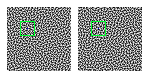
\includegraphics[width=0.5\linewidth]{content/simulatedAnnealing/Bilder/Permutation.png}
    \caption{Permutation}
    \label{pic:Permutation}
\end{figure}

\newpage

\begin{figure}[H]
    \centering 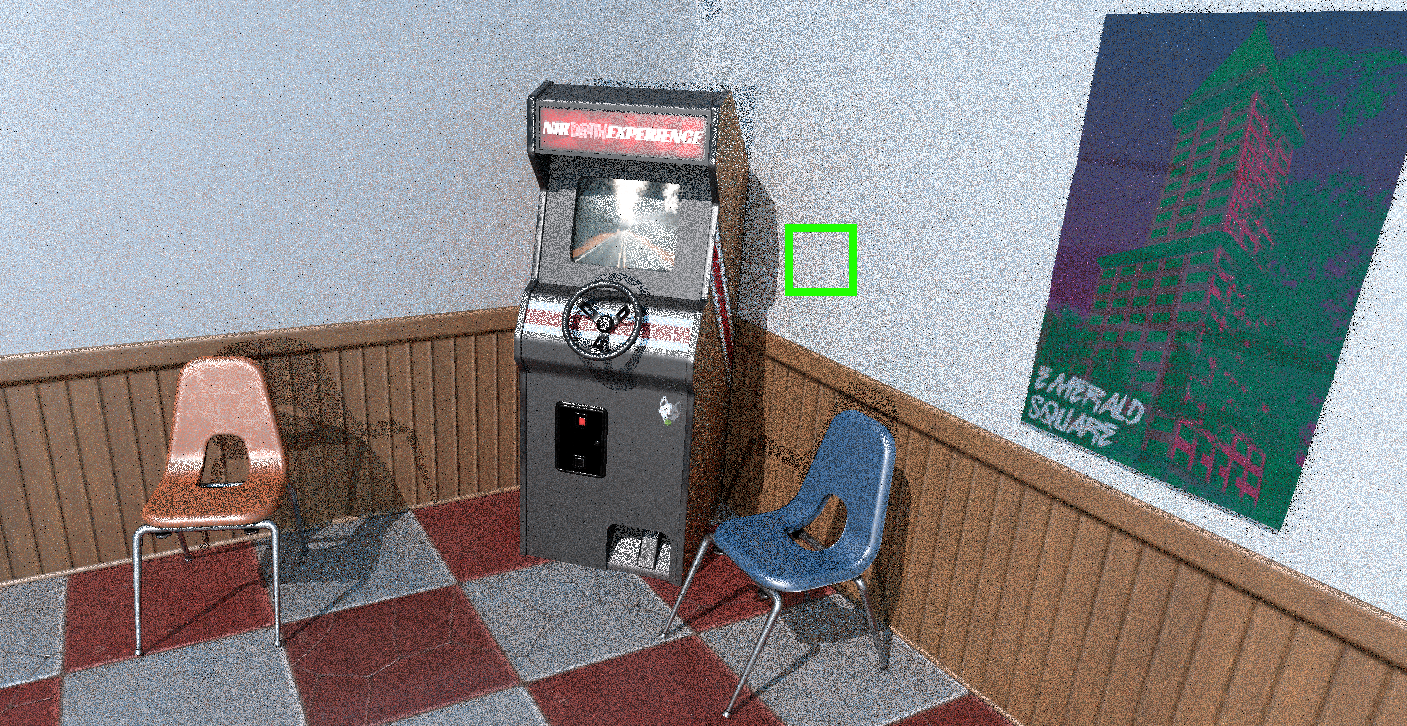
\includegraphics[scale=.25]{content/TemporalerAlg/Bilder/Retargeting/Szene/Szene1.png}
    \caption{Szene}
    \label{fig:Sorting_retarget_Szene_t1}
\end{figure}
%%%%%%%%%%%%%%%%%%%%%%%%%%%%%%%%%%%%%%%%%%%%%%%%%%%%%%%%%%%%%%%%%%%%%%%%%%%%%%%%%%%%%%%%%%%%%%%%%%%%%%
%%%%%%%%%%%%%%%%%%%%%%%%%%%%%%% second row; ausschnitt over time
%%%%%%%%%%%%%%%%%%%%%%%%%%%%%%%%%%%%%%%%%%%%%%%%%%%%%%%%%%%%%%%%%%%%%%%%%%%%%%%%%%%%%%%%%%%%%%%%%%%%%%  
\begin{figure}[H]
    \begin{tcolorbox}[boxrule=4pt,sharp corners=downhill,title=Retargeting]
    %%%%%%%%%%%%%%%%%%%%%%%%%%%%%%%%%%%%%%%%%%%%%%%%%%%%%%%%%%%%%%%%%%%%%%%%%%%%%%%%%%%%%%%%%%%%%%%%%%%%%%
    %%%%%%%%%%%%%%%%%%%%%%%%%%%%%%% first ausschnitt row
    %%%%%%%%%%%%%%%%%%%%%%%%%%%%%%%%%%%%%%%%%%%%%%%%%%%%%%%%%%%%%%%%%%%%%%%%%%%%%%%%%%%%%%%%%%%%%%%%%%%%%%  
    \begin{subfigure}[b]{0.2\textwidth}
        \centering
        
\includegraphics[width=\textwidth]{content/TemporalerAlg/Bilder/Retargeting/Ausschnitte/Ausschnitt1.png}
        \caption{t=1}
        \label{pic:sorting_retarget_t1}
    \end{subfigure}
    \begin{subfigure}[b]{0.2\textwidth}
        \centering
        
\includegraphics[width=\textwidth]{content/TemporalerAlg/Bilder/Retargeting/Spektren/Ausschnitt1.png}
        \subcaption{FFT t=1}
        \label{pic:sorting_retarget_t1_FFT}
    \end{subfigure}
    \begin{subfigure}[b]{0.1\textwidth}
        \hspace*{1cm}
    \end{subfigure}
    \begin{subfigure}[b]{0.2\textwidth}
        \centering
        
\includegraphics[width=\textwidth]{content/TemporalerAlg/Bilder/Retargeting/Ausschnitte/Ausschnitt5.png}
        \subcaption{FFT t=5}
        \label{pic:sorting_retarget_t5}
    \end{subfigure}
    \begin{subfigure}[b]{0.2\textwidth}
        \centering
        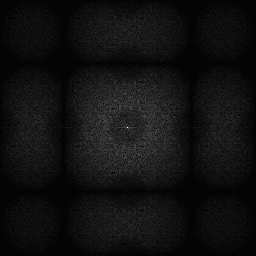
\includegraphics[width=\textwidth]{content/TemporalerAlg/Bilder/Retargeting/Spektren/Ausschnitt5.png}
        \subcaption{FFT t=5}
        \label{pic:sorting_t5_retarget_FFT}
    \end{subfigure}
    %%%%%%%%%%%%%%%%%%%%%%%%%%%%%%%%%%%%%%%%%%%%%%%%%%%%%%%%%%%%%%%%%%%%%%%%%%%%%%%%%%%%%%%%%%%%%%%%%%%%%%
    %%%%%%%%%%%%%%%%%%%%%%%%%%%%%%% second row; ausschnitt over time
    %%%%%%%%%%%%%%%%%%%%%%%%%%%%%%%%%%%%%%%%%%%%%%%%%%%%%%%%%%%%%%%%%%%%%%%%%%%%%%%%%%%%%%%%%%%%%%%%%%%%%%  
    \begin{subfigure}[b]{0.2\textwidth}
        \centering
        
\includegraphics[width=\textwidth]{content/TemporalerAlg/Bilder/Retargeting/Ausschnitte/Ausschnitt2.png}
        \caption{t=2}
        \label{pic:sorting_retarget_t2}
    \end{subfigure}
    \begin{subfigure}[b]{0.2\textwidth}
        \centering
        
\includegraphics[width=\textwidth]{content/TemporalerAlg/Bilder/Retargeting/Spektren/Ausschnitt2.png}
        \subcaption{FFT t=2}
        \label{pic:sorting_retarget_t2_FFT}
    \end{subfigure}
    \begin{subfigure}[b]{0.1\textwidth}
        \hspace*{1cm}
    \end{subfigure}
    \begin{subfigure}[b]{0.2\textwidth}
        \centering
        
\includegraphics[width=\textwidth]{content/TemporalerAlg/Bilder/Retargeting/Ausschnitte/Ausschnitt6.png}
        \subcaption{FFT t=6}
        \label{pic:sorting_retarget_t6}
    \end{subfigure}
    \begin{subfigure}[b]{0.2\textwidth}
        \centering
        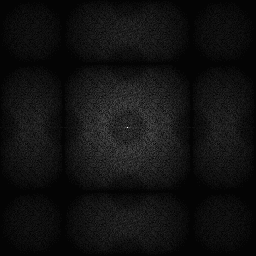
\includegraphics[width=\textwidth]{content/TemporalerAlg/Bilder/Retargeting/Spektren/Ausschnitt6.png}
        \subcaption{FFT t=6}
        \label{pic:sorting_retarget_t6_FFT}
    \end{subfigure}
    %%%%%%%%%%%%%%%%%%%%%%%%%%%%%%%%%%%%%%%%%%%%%%%%%%%%%%%%%%%%%%%%%%%%%%%%%%%%%%%%%%%%%%%%%%%%%%%%%%%%%%
    %%%%%%%%%%%%%%%%%%%%%%%%%%%%%%% third row; ausschnitt over time
    %%%%%%%%%%%%%%%%%%%%%%%%%%%%%%%%%%%%%%%%%%%%%%%%%%%%%%%%%%%%%%%%%%%%%%%%%%%%%%%%%%%%%%%%%%%%%%%%%%%%%%  
    \begin{subfigure}[b]{0.2\textwidth}
        \centering
        
\includegraphics[width=\textwidth]{content/TemporalerAlg/Bilder/Retargeting/Ausschnitte/Ausschnitt3.png}
        \caption{t=3}
        \label{pic:sorting_retarget_t3}
    \end{subfigure}
    \begin{subfigure}[b]{0.2\textwidth}
        \centering
        
\includegraphics[width=\textwidth]{content/TemporalerAlg/Bilder/Retargeting/Spektren/Ausschnitt3.png}
        \subcaption{FFT t=3}
        \label{pic:sorting_retarget_t3_FFT}
    \end{subfigure}
    \begin{subfigure}[b]{0.1\textwidth}
        \hspace*{1cm}
    \end{subfigure}
    \begin{subfigure}[b]{0.2\textwidth}
        \centering
        
\includegraphics[width=\textwidth]{content/TemporalerAlg/Bilder/Retargeting/Ausschnitte/Ausschnitt7.png}
        \subcaption{FFT t=7}
        \label{pic:sorting_retarget_t7}
    \end{subfigure}
    \begin{subfigure}[b]{0.2\textwidth}
        \centering
        
\includegraphics[width=\textwidth]{content/TemporalerAlg/Bilder/Retargeting/Spektren/Ausschnitt7.png}
        \subcaption{FFT t=7}
        \label{pic:sorting_retarget_t7_FFT}
    \end{subfigure}
    %%%%%%%%%%%%%%%%%%%%%%%%%%%%%%%%%%%%%%%%%%%%%%%%%%%%%%%%%%%%%%%%%%%%%%%%%%%%%%%%%%%%%%%%%%%%%%%%%%%%%%
    %%%%%%%%%%%%%%%%%%%%%%%%%%%%%%% 4th row; ausschnitt over time
    %%%%%%%%%%%%%%%%%%%%%%%%%%%%%%%%%%%%%%%%%%%%%%%%%%%%%%%%%%%%%%%%%%%%%%%%%%%%%%%%%%%%%%%%%%%%%%%%%%%%%%  
    \begin{subfigure}[b]{0.2\textwidth}
        \centering
        
\includegraphics[width=\textwidth]{content/TemporalerAlg/Bilder/Retargeting/Ausschnitte/Ausschnitt4.png}
        \caption{t=4}
        \label{pic:sorting_retarget_t4}
    \end{subfigure}
    \hspace*{0.1cm}
    \begin{subfigure}[b]{0.2\textwidth}
        \centering
        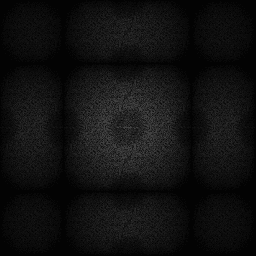
\includegraphics[width=\textwidth]{content/TemporalerAlg/Bilder/Retargeting/Spektren/Ausschnitt4.png}
        \subcaption{FFT t=4}
        \label{pic:sorting_retarget_t4_FFT}
    \end{subfigure}
    \end{tcolorbox}
    \caption{Retargeting ab t=1 aktiviert}
    \label{pic:Sorting_retarget_over_seven_frames} 
\end{figure}

\begin{figure}[H]
    \centering 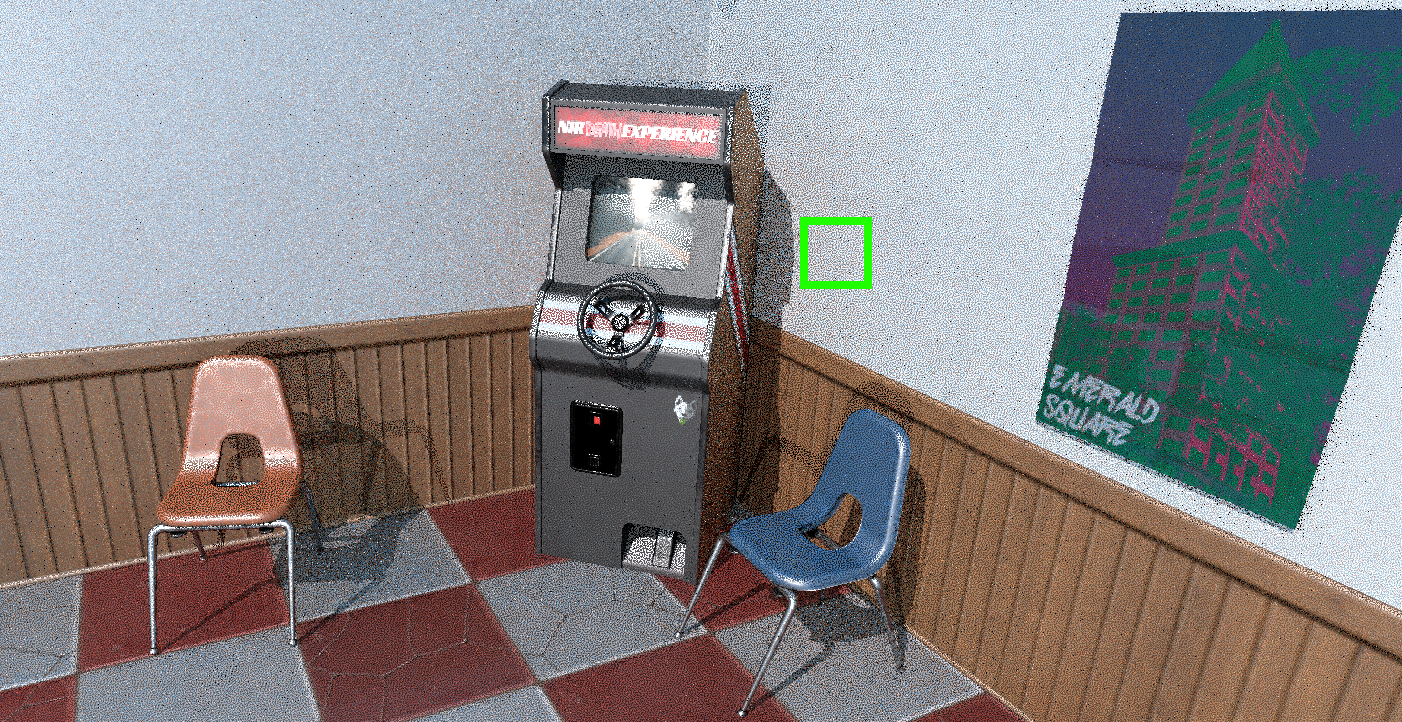
\includegraphics[scale=.25]{content/TemporalerAlg/Bilder/Retargeting/Szene/Szene7.png}
    \caption{Szene}
    \label{fig:Sorting_retarget_Szene_t7}
\end{figure}


\begin{itemize}
    \item[t=1-2] Die ersten beiden erzeugten Bilder lassen keine blue noise Eigenschaften erkennen.
                    Das typische weiße Rauschen ist zu erkennen und hat einen unbefriedigenden optischen Eindruck.
                     \par 
                    
    \item[t=3] Ab dem dritten Bild können wir eine \nameref{ch:Content1:sec:blue noise} Eigenschaft im Bild durch ein 
                bloßes Sortieren erkennen. Die daraus resultierende Steigerung der optisch wahrnehmbaren 
                Qualität, wie bereits in Arbeiten wie \cite{3288} besprochen, lässt sich gut erkennen. 
    \item[t=4-7] In den darauffolgenden Schritten ist eine zeitlich stabilere blue noise Verteilung zu erkennen.
                 Die Schwankungen zwischen den darauf folgenden Bildern wird geringer durch die vorherige 
                 Umsortierung zur nächsten blue noise Textur. 
\end{itemize}

%%%%%%%%%%%%%%%%%%%%%%%%%%%%%%%%%%%%%%%%%%%%%%%%%%%%%%%%%%%%%%%%%%%%%%%%%%%%%%%%%%%%%%%%%%%%%%%%%%%%%%
%%%%%%%%%%%%%%%%%%%%%%%%%%%%%%% Verdeutlichung der Akkumulation des Retargeting
%%%%%%%%%%%%%%%%%%%%%%%%%%%%%%%%%%%%%%%%%%%%%%%%%%%%%%%%%%%%%%%%%%%%%%%%%%%%%%%%%%%%%%%%%%%%%%%%%%%%%%

Zur Verdeutlichung der Bedeutung des zusätzlichen Retargeting zum vorherigen Sortierschritt:

\begin{figure}[H]
    
    \begin{tcolorbox}[sidebyside,title=Vergleich mit/ohne Retargeting]
        \paragraph{\hfill\colorbox{blue}{\textcolor{white}{nur Sorting}}}
        \centering
        \begin{subfigure}{0.5\textwidth}
            \centering
\includegraphics[width=\linewidth]{content/TemporalerAlg/Bilder/Sorting/Spektren/Ausschnitt7.png} 
            \caption{FFT reines Sorting}
            \label{fig:VergleichSorting}
        \end{subfigure}
    \tcblower
    \paragraph{\hfill\colorbox{blue}{\textcolor{white}{Sorting + Retargeting}}}
        \centering
        \begin{subfigure}{0.5\textwidth}
            \centering
\includegraphics[width=\linewidth]{content/TemporalerAlg/Bilder/Retargeting/Spektren/Ausschnitt7.png}
            \caption{FFT Sorting + Retargeting}
            \label{fig:VergleichRetargeting}
        \end{subfigure}
    \end{tcolorbox}
    \caption{Vergleich des jeweilig siebten Bildes reines Sorting und zusätzliches Retargeting}
    \label{fig:VergleichBild7}
\end{figure}

Über die Zeit lässt sich der zusätzliche Permutationschritt gut verdeutlichen. Das Spektrum des siebten gerenderten Bildes 
hat beim bloßen Sortieren (Bild \ref{fig:VergleichSorting}) keinen so starken Kontrast wie das Spektrum mit 
zusätzlichem Retargeting (Bild \ref{fig:VergleichRetargeting}). Die blue noise Umverteilungen Akkumulieren nicht so gut 
und führen zu dem verwischten Charakter. 